% Lecture Template for ME3023 -  Measurements in Mechanical Systems - Tennessee Technological University
% Spring 2020 - Summer 2020 - Fall 2020 - Spring 2021 - Summer 2021 - Fall 2023
% Tristan Hill, May 07, 2020 - June 12, 2020 - July 08, 2020 - Novemeber 02, 2020 - March 28, 2021 - May 25, 2021 - August 21, 2022 - September 02, 2023 - September 09, 2023

% Fall 2023 - condensing and streamlining lectures by combining topics into a single PDF under the module name
%			  this will simplify file and link management as well as make lectures easier to use in class
%			- added image/ to clean directory and reduce redundancy, specific to module for now  
% Fall  2024 - still converting, im slow ...

% Module Name: - Error and Uncertainty (previously toerr is human)
% Topic 1 - Accuracy and Error
% Topic 2 - Errors, Residuals, and Uncertainty
% Topic 3 - Repeatability and Testing

\documentclass[fleqn]{beamer} % for presentation (has nav buttons at bottom)
\usepackage{../measurements_lectures}

\author{ME3023 - Measurements in Mechanical Systems}

\newcommand{\MNUM}{?\hspace{2mm}} % module number 
\newcommand{\moduletitle}{Error and Uncertainty}

\newcommand{\sectionItitle}{Accuracy and Error}
\newcommand{\sectionIItitle}{Errors, Residuals, and Uncertainty}
\newcommand{\sectionIIItitle}{Repeatability and Testing}

\newcommand{\sectionIsubsectionItitle}{Accuracy and Error}
\newcommand{\sectionIsubsectionIItitle}{Estimating Error}
\newcommand{\sectionIsubsectionIIItitle}{Uncertainty Interval}
\newcommand{\sectionIsubsectionIVtitle}{GPS Activity}

\newcommand{\sectionIIsubsectionItitle}{Random and Systematic Errors}
\newcommand{\sectionIIsubsectionIItitle}{Dart Board Example}
\newcommand{\sectionIIsubsectionIIItitle}{Types of Errors}
\newcommand{\sectionIIsubsectionIVtitle}{Sample Uncertainty Data}

\newcommand{\sectionIIIsubsectionItitle}{Instrument Repeatability}
\newcommand{\sectionIIIsubsectionIItitle}{Conditions for Repeatability}
\newcommand{\sectionIIIsubsectionIIItitle}{Reproducibility and Instrument Uncertainty}
\newcommand{\sectionIIIsubsectionIVtitle}{---}

 \newcommand{\btVFill}{\vskip0pt plus 1filll}

% custom box
\newsavebox{\mybox}

\title{Lecture Module - \moduletitle}

\date{Mechanical Engineering\vspc Tennessee Technological University}

\begin{document}

	\lstset{language=MATLAB,basicstyle=\ttfamily\small,showstringspaces=false}

	\frame{\titlepage \center\begin{framed}\Large \textbf{Module \MNUM - \moduletitle}\end{framed} \vspace{5mm}}

	% Module Outline
	\begin{frame} 
		\large \textbf{Module \MNUM - \moduletitle} \vspace{3mm}\\

		\begin{itemize}
			\item Topic 1 - \hyperlink{sectionI}{\sectionItitle} \vspc % section I
			\item Topic 2 - \hyperlink{sectionII}{\sectionIItitle} \vspc % section II
			\item Topic 3 - \hyperlink{sectionIII}{\sectionIIItitle} \vspc % section III
		\end{itemize}

	\end{frame}

	% section I
	\section{\sectionItitle}\label{sectionI}

		% section I Outline
		\begin{frame} 
			\large \textbf{Topic 1 - \sectionItitle} \vspace{3mm}\\

			\begin{itemize}
				\item \hyperlink{sectionIsubsectionI}{\sectionIsubsectionItitle} \vspc %  section I subsection I
				\item \hyperlink{sectionIsubsectionII}{\sectionIsubsectionIItitle} \vspc % section I subsection II
				\item \hyperlink{sectionIsubsectionIII}{\sectionIsubsectionIIItitle} \vspc % section I subsection III
				\item \hyperlink{sectionIsubsectionIV}{\sectionIsubsectionIVtitle} \vspc % section I subsection IV
			\end{itemize}
		\end{frame}
		
		% section I subsection I 
		\subsection{\sectionIsubsectionItitle}\label{sectionIsubsectionI}

			\begin{frame}
				\frametitle{\sectionIsubsectionItitle}

				\bigskip		
				The exact value of a variable is called the \hspcu \hspc \hspcu. The value of the variables as indicated by a
				measurement system is called the \hspcu \hspc \hspcu. The \hspcu of a measurement refers to the
				closeness of agreement between the measured value and the true value. But the \hspcu \hspc \hspcu is rarely
				known \hspcu, and various influences, called \hspcu, have an effect on both of these values. So the
				concept of the \hspcu of a measurement is a \hspcu one. \vspcc

				\begin{framed}
					%\scalebox{1}{}$\hspace{10mm}{\RD error} = {\BL measured\hspace{1mm}value} - {\GR true\hspace{1mm}value} $}
				\end{framed}

				\btVFill
				{\tiny Text: Theory and Design of Mech. Meas.}
							
			\end{frame}

			\begin{frame}
				\frametitle{\sectionIsubsectionItitle}

				
					
			\end{frame}

		% section I subsection II
		\subsection{\sectionIsubsectionIItitle}\label{sectionIsubsectionII}

			\begin{frame}
				\frametitle{\sectionIsubsectionIItitle}

				The \hspcu \hspc \hspcu can be estimated but cannot be known  \hspcu. In practice a \hspcu value is used in place of the true value. We will discuss this again the the {\it Calibration Module}.

				\begin{framed}%\scalebox{1}{$\hspace{20mm} {\PR accuracy} =  \frac{|{\RD error}|}{{\BR reference\hspace{1mm}value}}\times 100 $}
				\end{framed}

				An estimate of error based using this value is sometimes referred to as \hspcu \hspc \hspcu. \vspc
						

		
			\end{frame}

			\begin{frame}
				\frametitle{\sectionIsubsectionIItitle}

				

			\end{frame}

			\begin{frame}

				


			\end{frame}


		% section I subsection III
		\subsection{\sectionIsubsectionIIItitle}\label{sectionIsubsectionIII}
			\begin{frame} 
				\frametitle{\sectionIsubsectionIIItitle}
				``The \hspcu is a numerical estimate of the possible range of the error in a measurement. In any
				measurement, the \hspcu is not known exactly since the true value is rarely known exactly. But based on
				available information, the operator might feel confident that the error is within certain bounds, a plus
				or minus range of the indicated reading. This is the assigned \hspcu.''\vspace{5mm}\\
				We will discuss this again the the {\it Uncertainty Module}.\vspace{10mm}\\

				{\tiny Text: Theory and Design of Mech. Meas.}
				

			\end{frame}	

			\begin{frame} 
				\frametitle{\sectionIsubsectionIIItitle}

				
			\end{frame}	

		% section I subsection IV
		\subsection{\sectionIsubsectionIVtitle}\label{sectionIsubsectionIV}	

			\begin{frame}
				\frametitle{\sectionIsubsectionIVtitle}

				\scriptsize
				{\bf Experiment}: We are going to collect data with the sensor suite on our phones. \vspc
				
				\begin{multicols}{2}
				    Sensor:
				    \begin{itemize}
				    	\item GPS - \href{https://en.wikipedia.org/wiki/File:ConstellationGPS.gif}{concept graphic} 
				    	\item \href{https://www.garmin.com/en-US/aboutgps/}{info from manufacturer}  
				    \end{itemize}

				    Logger Apps:
					\begin{itemize}
						\item \href{https://www.tszheichoi.com/sensorlogger}{sensorlogger (Android) - Kelvin Choi} \vspc
						\item \href{https://apps.apple.com/us/app/sensor-logger/id1531582925}{Sensor Logger (OSX) -Choi Tsz Hei}
					\end{itemize}

					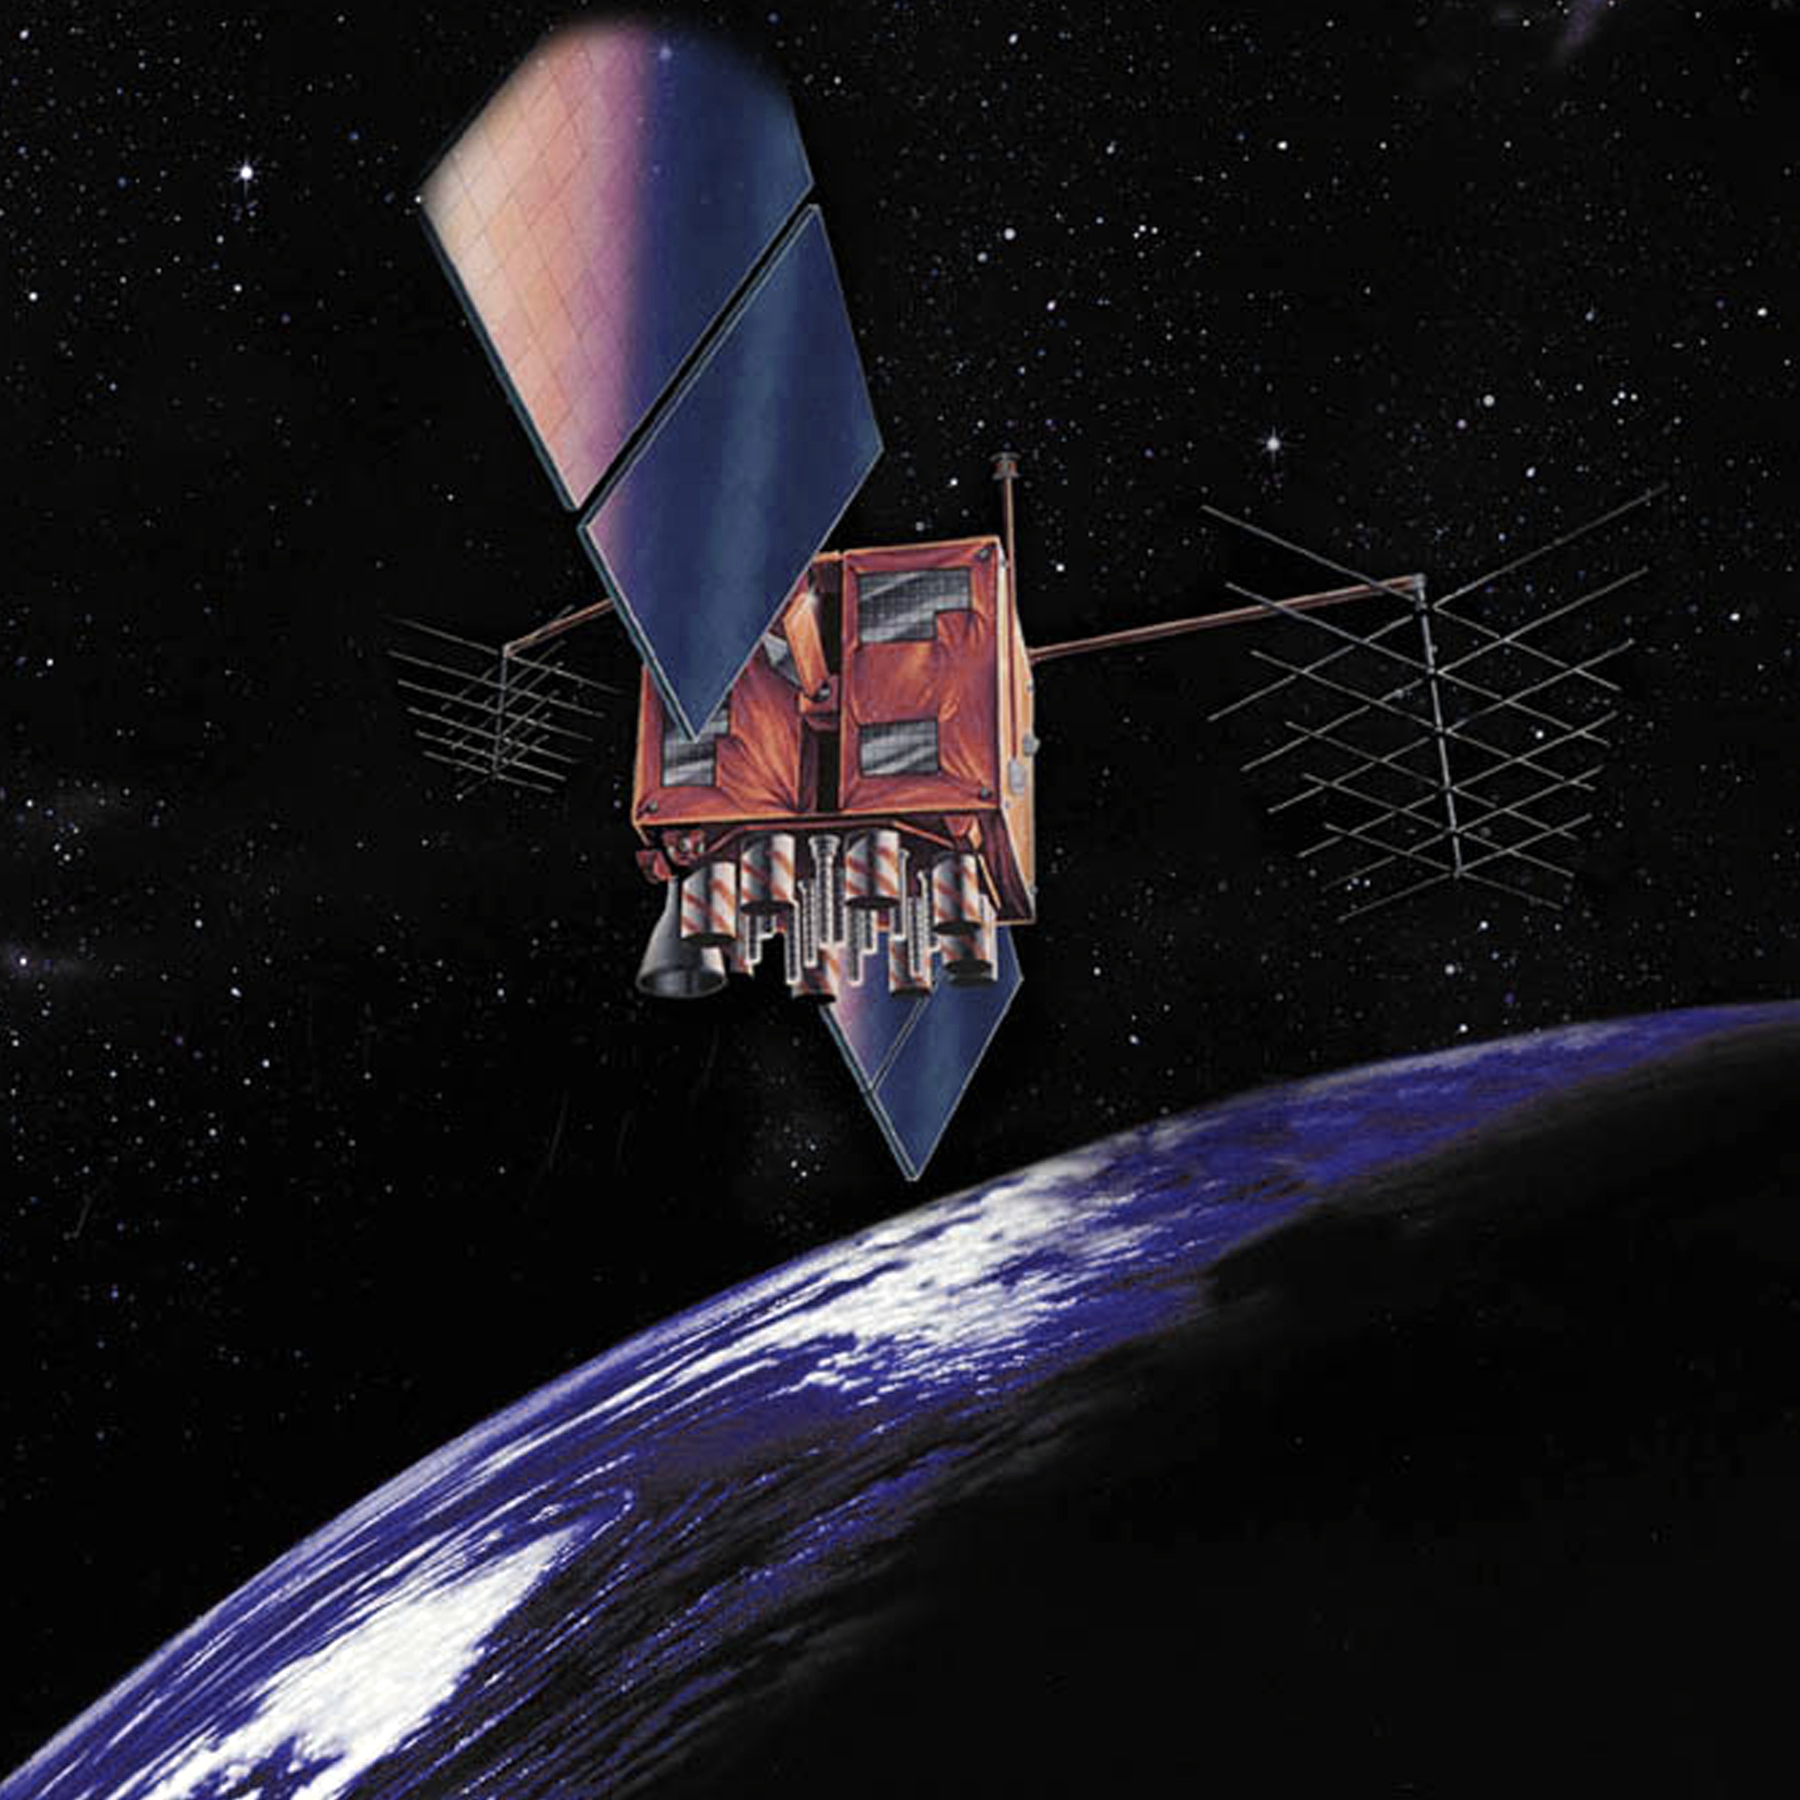
\includegraphics[scale=.075,angle=-90,origin=c]{images/GPS-IIR.jpeg}
					{\tiny Image:\href{https://en.wikipedia.org/wiki/Global_Positioning_System}{Wikipedia}}
				\end{multicols}	
				
			\end{frame}

			\begin{frame}
				\frametitle{\sectionIsubsectionIVtitle}
				\scriptsize
				{\bf Part 1 - Informed Prediction}: Generate data you expect the GPS in your phone to report. Show the data points on the graph to the right.  \\
				
				\begin{multicols}{2}
					\setlength{\tabcolsep}{20pt}
					\renewcommand{\arraystretch}{1.4}
					\begin{tabular}{|c|c|c|} \hline
					$i$ & $lat_i$ & $lon_i$ \\\hline
					  1  & &              \\ \hline
					  2  & &              \\ \hline
					  3  & &              \\ \hline
					  4  & &              \\ \hline
					  5  & &              \\ \hline

					\end{tabular}

					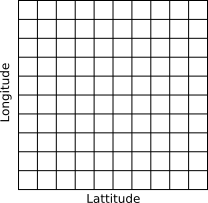
\includegraphics[scale=1]{images/lat_lon_grid.png}
					{\tiny Image: thill}
				\end{multicols}	

			\end{frame}

			\begin{frame}
				\frametitle{\sectionIsubsectionIVtitle}

				\scriptsize
				{\bf Part 2 - Measurement}: Record GPS from your phone. Show the data points on the graph to the right. You can use export feature in Sensor Logger to report the data.  \\
				
				\begin{multicols}{2}

					\setlength{\tabcolsep}{20pt}
					\renewcommand{\arraystretch}{1.4}
					\begin{tabular}{|c|c|c|} \hline
					$i$ & $lat_i$ & $lon_i$ \\\hline
					  1  & &              \\ \hline
					  2  & &              \\ \hline
					  3  & &              \\ \hline
					  4  & &              \\ \hline
					  5  & &              \\ \hline
					  6  & &              \\ \hline
					  7  & &              \\ \hline
					  8  & &              \\ \hline
					  8  & &              \\ \hline		
					  9  & &              \\ \hline
		             10  & &              \\ \hline
					\end{tabular}

					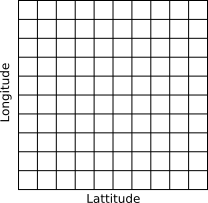
\includegraphics[scale=1]{images/lat_lon_grid.png}
					{\tiny Image: thill}
				\end{multicols}	
				
			\end{frame}
	
			\begin{frame}
				\frametitle{\sectionIsubsectionIVtitle}

				\scriptsize
				{\bf Part 3 - Analysis/Results/Conclusions}: Compare and contrast the two sets of data. What conclusions can you make about your predictions or the sensor data?
				\begin{multicols}{2}

					\begin{itemize}
						\item Were the predictions reasonable? \\
						\item What type of error is present in the recorded data? \\
						\item What should be used as a reference for this data? \\ 
					\end{itemize}
					
					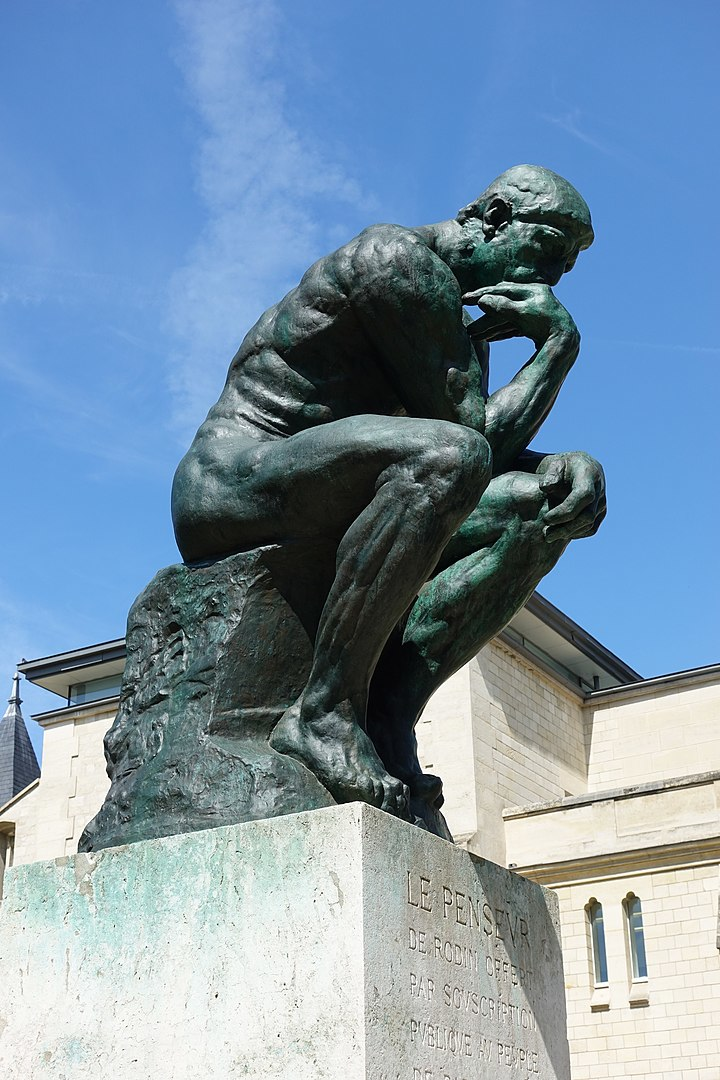
\includegraphics[scale=.1]{images/thinker_rodin.png}
					
\includegraphics[scale=.25]{images/thinker_dc_comics.png}
					{\tiny Image: \href{https://en.wikipedia.org/wiki/Thinker_(DC_Comics)}{wikipedia}}
					{\tiny Image: \href{https://en.wikipedia.org/wiki/The_Thinker}{wikipedia}}
				\end{multicols}	
				
			\end{frame}


			\begin{frame}
				\frametitle{\sectionIsubsectionIVtitle}
				Deliverables:
				\begin{itemize}
					\item some stuff
					\item and some more stuff
				\end{itemize}
				


			\end{frame}

	% Section II
	\section{\sectionIItitle}\label{sectionII}

		% section II Outline
		\begin{frame}
			\large \textbf{Topic 2 - \sectionIItitle} \vspace{3mm}\\

			\begin{itemize}
				\item \hyperlink{sectionIIsubsectionI}{\sectionIIsubsectionItitle} \vspc %  section II subsection I
				\item \hyperlink{sectionIIsubsectionII}{\sectionIIsubsectionIItitle} \vspc % section II subsection II
				\item \hyperlink{sectionIIsubsectionIII}{\sectionIIsubsectionIIItitle} \vspc % section II subsection III
				\item \hyperlink{sectionIIsubsectionIV}{\sectionIIsubsectionIVtitle} \vspc % section II subsection IV
			\end{itemize}

		\end{frame}

		% section II subsection I
		\subsection{\sectionIIsubsectionItitle}\label{sectionIIsubsectionI}

			\begin{frame}[label=sectionIIsubsectionI]
				\frametitle{\sectionIIsubsectionItitle}

				"Errors are effects that cause a  measured value to differ from its true value. \hspcu error causes a
				\hspcu variation in measured values found during repeated measurements of a variable. \vspc
				\hspcu error causes an offset between the mean value of the data set and its true value. Both \hspcu and
				\hspcu errors affect a system's accuracy."

				\vspace{10mm}
				{\tiny Text: Theory and Design of Mech. Meas.}

			\end{frame}

		    \begin{frame}[label=sectionIIsubsectionI]
				\frametitle{\sectionIIsubsectionItitle}





			\end{frame}	

		% section II subsection II
		\subsection{\sectionIIsubsectionIItitle}\label{sectionIIsubsectionII}

			\begin{frame}
				\frametitle{\sectionIIsubsectionIItitle}
				"The concept of accuracy and the effects of \hspcu and \hspcu errors in instruments
				and measurement systems can be illustrated by the throw of darts."

				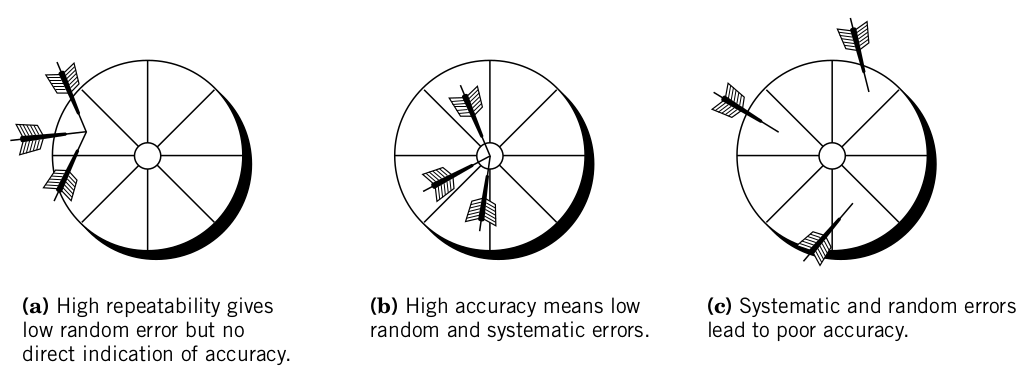
\includegraphics[scale=.20]{images/dart_throw.png}

				The ability of a measurement system to indicate the same value on repeated but independent
				application of the same input provides a measure of the instrument \hspcu."

				{\tiny Text, Image: Theory and Design of Mech. Meas.}

			\end{frame}

		% section II subsection III
		\subsection{\sectionIIsubsectionIIItitle}\label{sectionIIsubsectionIII}

			\begin{frame}
				\frametitle{\sectionIIsubsectionIIItitle}

				Common categories of errors in measurements are shown below. This is not an exhaustive list.  

				\begin{itemize}
					
					\item Linearity Error \vspc
					\item Sensitivity \vspc
					\item Zero (offset) Error \vspc
					\item Hysteresis Error \vspc
					\item Overall Instrument Error \vspc
				\end{itemize}

				\[u_c=\sqrt{u_1^2+u_2^2+...+u_M^2}\]

			\end{frame}		

			\begin{frame}
				\frametitle{\sectionIIsubsectionIIItitle}

				

			\end{frame}

			\begin{frame}
				\frametitle{\sectionIIsubsectionIIItitle}

			\end{frame}

			\begin{frame}
			\frametitle{\sectionIIsubsectionIIItitle}





			\end{frame}

		% section II subsection IV 
		\subsection{\sectionIIsubsectionIVtitle}\label{sectionIIsubsectionIV}

			\begin{frame}
				\frametitle{\sectionIIsubsectionIVtitle}

				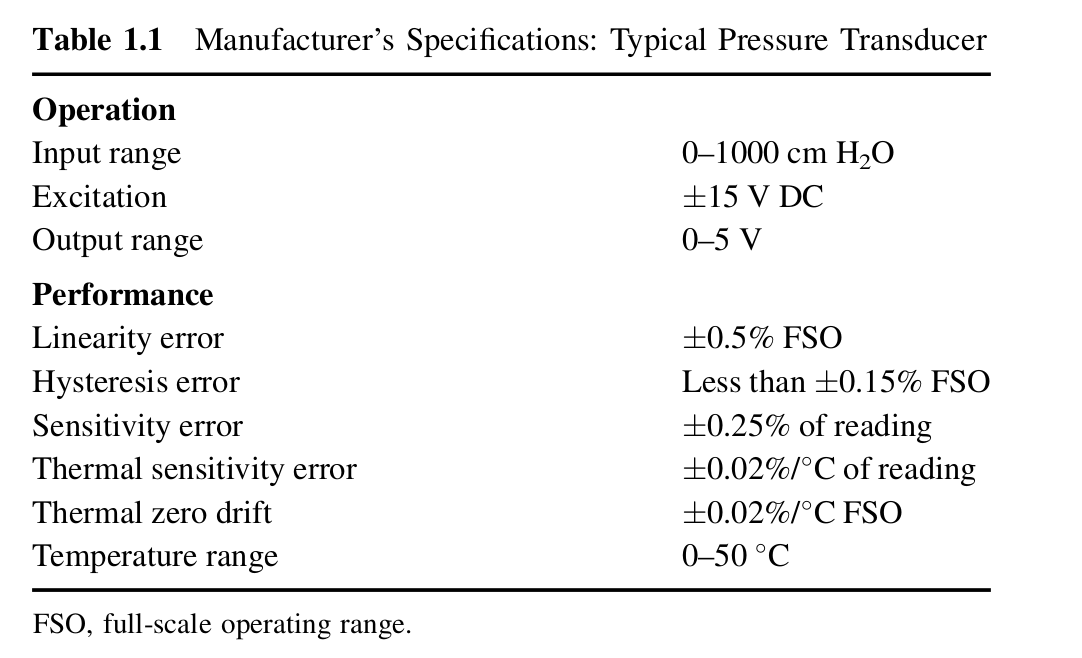
\includegraphics[scale=.22]{images/sample_uncertainties.png}

				{\tiny Text, Image, Data: Theory and Design of Mech. Meas.}


			\end{frame}

			\begin{frame}
				\frametitle{\sectionIIsubsectionIVtitle}




			\end{frame}

			\begin{frame}

			


			\end{frame}


		
	% Section III
	\section{\sectionIIItitle}\label{sectionIII}

		% section III Outline
		\begin{frame}
			\large \textbf{Topic 3 - \sectionIIItitle} \vspace{3mm}\\

			\begin{itemize}
				\item \hyperlink{sectionIIIsubsectionI}{\sectionIIIsubsectionItitle} \vspc %  section III subsection I
				\item \hyperlink{sectionIIIsubsectionII}{\sectionIIIsubsectionIItitle} \vspc % section III subsection II
				\item \hyperlink{sectionIIIsubsectionIII}{\sectionIIIsubsectionIIItitle} \vspc % section III subsection III
				\item \hyperlink{sectionIIIsubsectionIV}{\sectionIIIsubsectionIVtitle} \vspc % section III subsection IV
			\end{itemize}

		\end{frame}

		% section III subsection I
		\subsection{\sectionIIIsubsectionItitle}\label{sectionIIIsubsectionI}

			\begin{frame}
				\frametitle{\sectionIIIsubsectionItitle}

				
				``The ability of a measurement system to indicate the same value on repeated but independent
				application of the same input provides a measure of the instrument {\PN repeatability}. Specific claims of
				{\PN repeatability} are based on multiple calibration tests (replication) performed within a given lab on the
				particular unit.'' \vspc

				\begin{framed}\hspace{10mm}\scalebox{1}{$\%u_{R_{max}}=\frac{2s_x}{r_0}\times100$}\end{framed}

				\vspace{10mm}

				{\tiny Text: Theory and Design of Mech. Meas.}
				
			\end{frame}

			\begin{frame}
				\frametitle{\sectionIIIsubsectionItitle}
		
			\end{frame}

		% section III subsection II
		\subsection{\sectionIIIsubsectionIItitle}\label{sectionIIIsubsectionII}	

			\begin{frame}
				\frametitle{\sectionIIIsubsectionIItitle}

				The following conditions need to be fulfilled in the establishment of repeatability:
				\begin{itemize}

					\item the same experimental tools
					\item the same observer
					\item the same measuring instrument, used under the same conditions
					\item the same location
					\item repetition over a short period of time.
					\item same objectives

				\end{itemize}
				\vspace{5mm}
				{\tiny Text: \href{https://en.wikipedia.org/wiki/Repeatability}{Wikipedia(NIST)} }

			\end{frame}

		% section III subsection III
		\subsection{\sectionIIIsubsectionIIItitle}\label{sectionIIIsubsectionIII}

			\begin{frame}
				\frametitle{\sectionIIIsubsectionIIItitle}

				``The term {\GR reproducibility}, when reported in instrument specifications, refers to the closeness of
				agreement in results obtained from duplicate tests carried out under similar conditions of
				measurement ... \vspcc

				... The term {\PR instrument precision}, when reported in instrument specifications, refers to a random
				uncertainty based on the results of separate repeatability tests.'' \vspace{10mm} \\

				{\tiny Text: Theory and Design of Mech. Meas.}
		
			\end{frame}

			\begin{frame}
				\frametitle{\sectionIIIsubsectionIIItitle}



			\end{frame}

		% section III subsection IV
		\subsection{\sectionIIIsubsectionIVtitle}\label{sectionIIIsubsectionIV}	

			\begin{frame}
				\frametitle{\sectionIIIsubsectionIVtitle}

			


			\end{frame}

			\begin{frame}
				\frametitle{\sectionIIIsubsectionIVtitle}
				


			\end{frame}

\end{document}





